\documentclass{beamer}
\usepackage[utf8]{inputenc}

\usetheme{Madrid}
\usecolortheme{default}

\usepackage{amsmath,amssymb,amsfonts}
\usepackage{graphicx}
\usepackage{tikz}

\setbeamertemplate{page number in head/foot}[totalframenumber]

%------------------------------------------------------------
\title{Optimisation}
\date{March 25, 2026}

\author 
{Bhoomika V - EE25BTECH11015}

%------------------------------------------------------------

\begin{document}

\frame{\titlepage}

%------------------------------------------------------------
\begin{frame}{Question}
Item P is made from components Q and R.  

Item Q is made from S and T.  

Lead times (weeks):
\[
P=2,\; Q=3,\; R=10,\; S=5,\; T=6
\]

The lead time (in weeks) needed to respond to a customer order for item P is:

\begin{enumerate}
\item[(a)] 10
\item[(b)] 11
\item[(c)] 12
\item[(d)] 26
\end{enumerate}

\hfill (2007 PI)
\end{frame}

%------------------------------------------------------------
\begin{frame}{Product Structure}

\centering
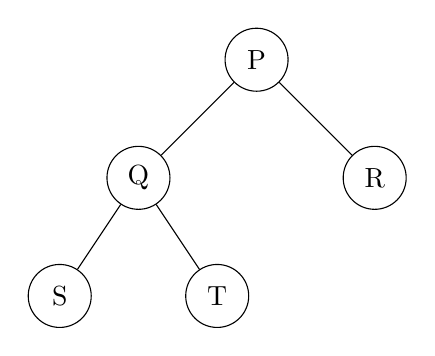
\begin{tikzpicture}[level distance=1.5cm,
every node/.style={circle,draw,minimum size=0.8cm},
level 1/.style={sibling distance=3cm},
level 2/.style={sibling distance=2cm}]

\node {P}
    child {node {Q}
        child {node {S}}
        child {node {T}}
    }
    child {node {R}};

\end{tikzpicture}

\end{frame}

%------------------------------------------------------------
\begin{frame}{Concept}
\begin{itemize}
\item Total lead time = Longest path from leaf to final product
\item All components must be ready before assembly
\item Hence, take the \textbf{maximum path time}
\end{itemize}
\end{frame}

%------------------------------------------------------------
\begin{frame}{Path Calculations}

\textbf{Path 1: } $S \rightarrow Q \rightarrow P$
\[
5 + 3 + 2 = 10
\]

\vspace{0.3cm}

\textbf{Path 2: } $T \rightarrow Q \rightarrow P$
\[
6 + 3 + 2 = 11
\]

\vspace{0.3cm}

\textbf{Path 3: } $R \rightarrow P$
\[
10 + 2 = 12
\]

\end{frame}

%------------------------------------------------------------
\begin{frame}{Final Calculation}

\[
\max(10,\;11,\;12) = 12
\]

\end{frame}

%------------------------------------------------------------
\begin{frame}{Final Answer}

\[
\boxed{12\ \text{weeks}}
\]

Correct Option: (c)

\end{frame}

%------------------------------------------------------------

\end{document}
